\chapter{Conclusion and Future Work}
\section{Summary of Contributions}

This research presents a Neural-Assisted Feature Matching (NAFM) framework
specifically designed to address the computational bottlenecks inherent in
traditional feature matching methods for real-time gaming applications. The
work demonstrates that the latter, while robust, impose significant latency
constraints that are incompatible with high-frame-rate gaming environments
where millisecond-level processing is critical.

The primary contribution lies in the development of a domain-specific
optimization of the XFeat architecture through a teacher-student learning
paradigm. Unlike previous approaches that rely on generic computer vision
datasets, this work creates a synthetic training framework tailored to gaming
scenarios. The synthetic dataset generation pipeline addresses unique
challenges in gaming environments, including semi-transparent UI elements,
dynamic lighting conditions, and the need for precise icon localization across
varying background complexities. Through systematic experimentation with 50,000
carefully constructed training samples using over 5,000 gaming template, the
research establishes that gaming-specific data synthesis significantly
outperforms generic training approaches for our specific use case.

The investigation of multiple teacher-student configurations reveals
counterintuitive findings about supervisory signal selection. While
neural-based teachers like ALIKE initially appeared promising due to their
modern architecture, the systematic evaluation demonstrates that classical SIFT
supervision (Variant C) provides superior learning outcomes for this specific
domain. This finding challenges the assumption that newer neural approaches
automatically translate to better teaching signals and highlights the
importance of domain-specific evaluation in teacher-student frameworks.

Performance analysis reveals substantial computational improvements while
maintaining practical accuracy levels. The optimized model achieves:
\begin{itemize}
    \item 12.4x speedup over traditional SIFT-CPU implementation
    \item 81.65\% total loss reduction during training convergence
    \item 199.4\% improvement in fine-grained matching accuracy
    \item 5.2\% in total evaluation accuracy compared to XFeat
    \item Maintained real-time processing capabilities on CPU-only systems
\end{itemize}

The work establishes a comprehensive evaluation framework that quantifies the
fundamental speed-accuracy trade-offs in feature matching systems. Through
detailed benchmarking across SIFT, XFeat-GPU, and XFeat-CPU implementations,
the research demonstrates that while neural approaches deliver
order-of-magnitude speedups, they require careful optimization to maintain the
match quality necessary for reliable gaming applications.

However, the research also identifies significant limitations that constrain
immediate deployment. The 60.9\% degradation in coarse accuracy performance
compared to baseline models indicates that the optimization process may have
introduced domain-specific biases that reduce generalization capability.
Additionally, the reliance on synthetic training data, while computationally
efficient, raises questions about real-world robustness that require extensive
validation in production gaming environments. The work acknowledges these
constraints and provides a foundation for addressing them in future iterations
of the system.
\section{Limitations}

This research faces several fundamental constraints that significantly impact
both the scope of investigation and the practical applicability of the proposed
neural-assisted feature matching framework. These limitations stem from data
availability challenges, computational resource constraints, and inherent
incompatibilities with existing computer vision benchmarks.

The most critical limitation arises from the scarcity of suitable gaming icon
templates available through public repositories or online sources. Unlike
general computer vision tasks where extensive datasets like ImageNet or COCO
provide thousands of labeled examples across diverse categories,
gaming-specific UI elements are typically proprietary assets protected by
intellectual property rights. Game developers and publishers rarely release
their visual assets publicly, creating a fundamental data acquisition
bottleneck. This constraint forced the research to rely on a manually curated
collection of no more than 5000 gaming icons, sourced primarily through web
scraping and fair-use extraction from publicly available gameplay footage. The
limited template diversity introduces potential bias in the learned feature
representations and raises serious questions about generalizability across
different gaming titles, art styles, and UI design paradigms.

The incompatibility with established computer vision datasets presents another
fundamental challenge that constrains methodological approaches. Standard
feature matching benchmarks like MegaDepth are designed for 3D scene
understanding tasks and require comprehensive geometric information including
depth maps, camera intrinsic parameters, pose matrices, and multi-view
correspondences. These data structures are entirely irrelevant to the 2D gaming
interface context, where UI elements exist in screen space without meaningful
depth relationships or camera geometry. This mismatch necessitated the complete
abandonment of proven evaluation protocols and the development of entirely
synthetic training pipelines, which inherently lack the visual complexity and
authenticity of real-world scenarios.

The reliance on synthetic data generation represents a significant
methodological compromise that undermines the ecological validity of the
research findings. While real-world gaming footage would provide authentic
training scenarios with genuine lighting conditions, rendering artifacts, and
visual complexity, the manual annotation requirements for such data prove
prohibitively expensive and time-consuming. Each frame of gameplay footage
would require precise keypoint labeling, correspondence mapping between
template icons and scene instances, geometric transformation annotation, and
extensive quality validation. Given that modern games render at 60+ frames per
second with constantly changing UI states, the annotation workload scales
exponentially with dataset size. A modest dataset of 10,000 annotated
correspondences would require hundreds of hours of expert annotation time,
costs that far exceed the resources available for this internship project.

Computational resource limitations imposed severe restrictions on the
experimental scope throughout this investigation. Training computer vision
models on a single GPU architecture creates substantial time penalties, with
each complete training run requiring 1-3 days to reach convergence depending on
the model complexity and dataset size, then 1-2 days to evaluate and study
findings. This extended training duration severely constrains the number of
architectural variations, hyperparameter configurations, and ablation studies
that can be practically explored within the project timeline. The reported
experiments represent only a small subset of the possible design space, leaving
critical questions about optimal network architectures, loss function
weighting, and data augmentation strategies largely unexplored.

The GPU memory constraints further limit batch sizes and model complexity,
potentially impacting training stability and final performance. With only 24GB
of available GPU memory, batch sizes were restricted to 10 samples, which may
be suboptimal for stable gradient estimation in deep learning contexts where
larger batches typically improve convergence properties. Additionally, the
inability to conduct parallel experiments across multiple GPUs means that
comparative studies between different approaches require sequential execution,
multiplying the already substantial time requirements.

These computational limitations become particularly restrictive when conducting
teacher-student experiments, where multiple models must be trained in sequence.
Each teacher-student pair evaluation requires training the teacher model,
generating pseudo-labels on the training set, and then training the student
model—effectively tripling the computational cost compared to single-model
experiments. This constraint severely limited the exploration of different
teacher architectures and prevented comprehensive ablation studies that would
have strengthened the experimental validation.

The narrow experimental scope resulting from these constraints means that many
critical research questions remain unanswered. The optimal balance between
synthetic and real data, the impact of different data augmentation strategies,
the effectiveness of various teacher model architectures, and the robustness
across different gaming genres all require extensive additional investigation
that was not feasible within the available resource constraints.
\section{Future Work}
\subsection{Introduction of Synthetic 3D data}
Coming late at the end of the project, the introduction of synthetic 3D data
presents a promising avenue for enhancing the training dataset, especially that
the chosen model is conceived with 3D information in mind. By incorporating 3D
assets and environments, we can create more realistic training scenarios that
better capture the complexities of real-world gaming interfaces. This could
involve generating 3D models of gaming icons and environments, then rendering
them from various angles and scales to create a diverse set of training
examples.
\subsubsection{Variant D}
This variation would be focused on creating a fully 3D-rendered environment
where the icons can be placed and interacted with in a more dynamic way. Our
first idea would be to synthesize a \textbf{pose matrix}, an \textbf{intrinsic
    camera matrix} and a depth map for each generated sample. The idea is to build
a pose matrix in correspondence with the rotation and translation of the icon,
on which the hypothetical camera is centered. So if we were to rotate the icon
by a certain angle $\theta$, and displacing it by a certain coordinates
$(t_x,t_y)$, we can compute the corresponding changes in the pose matrix to
reflect the new position and orientation of the icon in 3D space as if our icon
was to be a real object placed in a 3D environment.
\[
    P =
    \begin{bmatrix}
        R & t \\
        0 & 1
    \end{bmatrix}
\]
where $R$ is a $3\times3$ rotation matrix and $t$ is a $3\times1$ translation
vector. $t$ is computed as follows:
\[
    t =
    \begin{bmatrix}
        t_x \\
        t_y \\
        d
    \end{bmatrix}
\]
{\footnotesize * where $d$ is the depth value associated with the icon's position}\\
and $R$, Rotation component for rotation around Z-axis (assuming 2D rotation only):
\[
    R =
    \begin{bmatrix}
        \cos(\theta) & -\sin(\theta) & 0 \\
        \sin(\theta) & \cos(\theta)  & 0 \\
        0            & 0             & 1
    \end{bmatrix}
\] \\
The complete pose matrix would then translate to:
\[
    P_{icon} =
    \begin{bmatrix}
        \cos(\theta) & -\sin(\theta) & 0 & t_x \\
        \sin(\theta) & \cos(\theta)  & 0 & t_y \\
        0            & 0             & 1 & d   \\
        0            & 0             & 0 & 1
    \end{bmatrix}
\] \\
or:
\[
    P_{camera} =
    \begin{bmatrix}
        \cos(-\theta) & -\sin(-\theta) & 0 & -t_x \\
        \sin(-\theta) & \cos(-\theta)  & 0 & -t_y \\
        0             & 0              & 1 & -d   \\
        0             & 0              & 0 & 1
    \end{bmatrix}
\]\\
And we would use generate a 3D depth map from the camera's perspective by setting the icon as the foreground, an object between the camera and the background, we would give our icon a distance that corresponds to its scaling factor (an upscaling would mean a smaller distance, and a downscaling would mean a larger distance). The background would be set to a fixed distance, and the camera's intrinsic matrix would be set to a fixed value. This would allow us to create clear distinctions between the icon and the background, as when used without an explicit depth, we would not be able to distinguish between the icon and the background, especially in cases where the icon has similar colors and features to the background.
\begin{figure}[htbp]
    \centering
    \begin{subfigure}{0.48\textwidth}
        \centering
        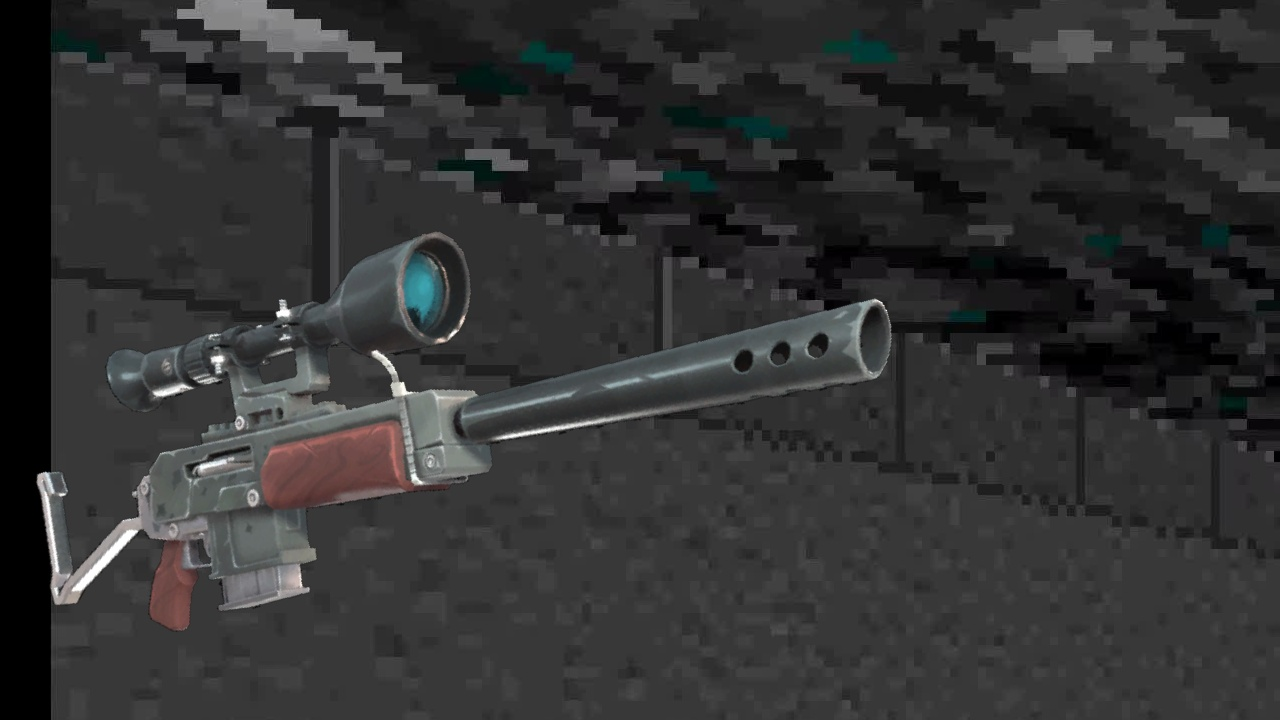
\includegraphics[width=\textwidth]{ressources/00009.jpg}
        \caption{First image caption}
        \label{fig:first-image}
    \end{subfigure}
    \hfill
    \begin{subfigure}{0.48\textwidth}
        \centering
        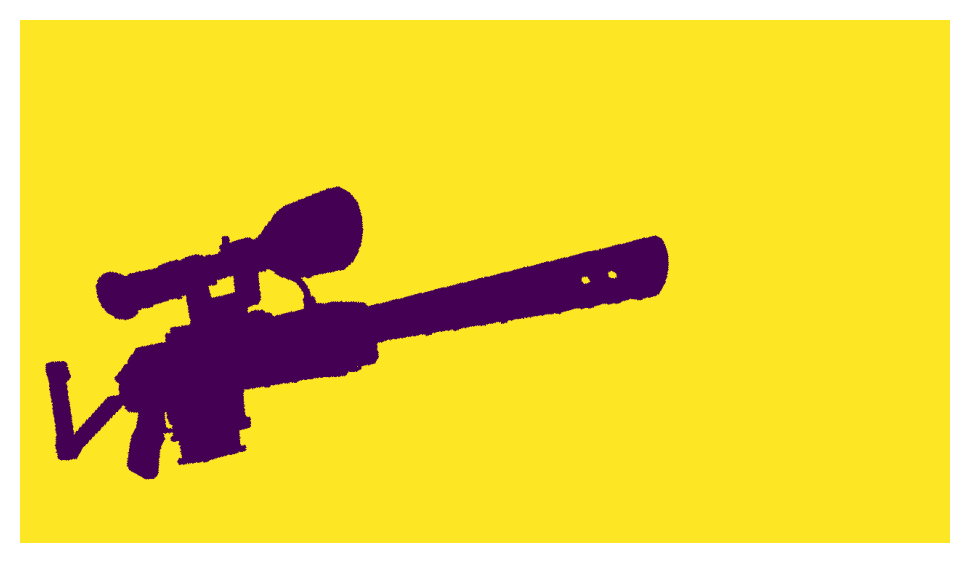
\includegraphics[width=\textwidth]{ressources/depth_map.png}
        \caption{Second image caption}
        \label{fig:second-image}
    \end{subfigure}
    \caption{Overall figure caption describing both images}
    \label{fig:double-image}
\end{figure}
\subsection{Better Matching Criterion}
The current matching criterion relies on the ratio of inliers to features
within the detected bounding box, but this approach exhibits several critical
limitations that compromise its reliability. When RANSAC filtering produces
weak results—either due to insufficient keypoints or low-quality
correspondences—the criterion becomes susceptible to both false positives and
false negatives. The fundamental issue stems from the criterion's inability to
distinguish between meaningful geometric consistency and coincidental spatial
clustering. False positives occur when background keypoints happen to fall
within the bounding box boundaries, artificially inflating the inlier count
despite lacking genuine correspondence to the target icon. Conversely, true
matches may be rejected when legitimate icon features are sparse or when RANSAC
fails to identify sufficient inliers, even though the underlying
correspondences are geometrically valid. This binary approach also ignores the
spatial distribution quality of matches. A few highly concentrated inliers in
one corner of the bounding box receive the same confidence score as evenly
distributed matches across the entire icon region, despite the latter providing
stronger evidence of correct detection. Future work should explore multi-factor
matching criteria that incorporate:
\begin{itemize}
    \item \textbf{Geometric consistency measures} beyond simple inlier counting, such as evaluating the uniformity of keypoint distribution across the detected region and assessing the coherence of local geometric transformations between matched features.
    \item \textbf{Descriptor quality assessment} that weighs matches based on their descriptor similarity scores rather than treating all correspondences equally, allowing high-confidence matches to carry more influence in the final decision.
    \item \textbf{Spatial relationship validation} that examines the structural relationships between keypoints, ensuring that matched features maintain expected relative positions and orientations consistent with the target icon's geometry.
\end{itemize}
These enhancements would address the current criterion's oversimplification while maintaining computational efficiency suitable for real-time gaming applications.

\subsection{Real-World Testing and Validation}
Real-world validation requires deploying the system on diverse gaming content across multiple titles and genres to assess performance under actual operating conditions. The testing framework should capture live gameplay footage at various frame rates and resolutions, measuring detection accuracy, false positive rates, and computational overhead during extended gaming sessions. Critical evaluation metrics include the system's ability to maintain real-time performance during graphically intensive scenes, robustness to UI scaling and transparency effects, and consistency across different lighting conditions and visual styles. The validation process must also examine failure modes, such as performance degradation during rapid scene transitions or when multiple UI elements appear simultaneously, to establish reliable operating parameters for production deployment.

\section{Personal Reflection on the Internship Experience}
\subsection{Assessment of the Position and Company}
The internship at SteelSeries provided valuable exposure to applied computer vision research within a gaming industry context. Working on neural-assisted feature matching offered hands-on experience with modern deep learning frameworks while addressing real computational constraints in production software. The company's commitment to maintaining high-performance gaming software created a challenging environment that demanded practical engineering solutions rather than purely academic approaches.
The technical mentorship was substantial, with access to both domain expertise in real-time software and guidance on deep learning implementation. The six-month internship period, while sufficient for proof-of-concept development, highlighted the extended validation cycles necessary for production-ready computer vision systems.
\subsection{Conclusion}
This work contributes to a larger shift toward neural acceleration of classical computer vision algorithms, particularly in resource-constrained environments. The findings suggest that domain-specific optimization can yield significant performance improvements, but also reveal the complexity of replacing well-established methods like SIFT in production systems. The teacher-student framework demonstrated here could extend beyond gaming applications to other real-time vision tasks where classical methods create computational bottlenecks.
The research exposes fundamental questions about the trade-offs between computational efficiency and reliability in computer vision systems. While neural approaches offer compelling speed advantages, the degradation in certain accuracy metrics underscores the need for careful evaluation frameworks that go beyond simple performance benchmarks. Future work in this area will likely need to address the generalization gap between synthetic training data and real-world deployment scenarios, potentially through improved domain adaptation techniques or hybrid classical-neural architectures that preserve the reliability advantages of traditional methods while incorporating the efficiency gains of modern neural networks
The internship experience at SteelSeries has been instrumental in shaping my understanding of the practical applications of computer vision in the industry. The challenges faced during the project underscored the importance of robust testing and validation methodologies. Moving forward, I am excited to explore the broader implications of neural-assisted traditional methods and their potential to enhance current solutions.
